% $Header: /home/vedranm/bitbucket/beamer/solutions/conference-talks/conference-ornate-20min.en.tex,v 90e850259b8b 2007/01/28 20:48:30 tantau $

\documentclass{beamer}

% This file is a solution template for:

% - Talk at a conference/colloquium.
% - Talk length is about 20min.
% - Style is ornate.



% Copyright 2004 by Till Tantau <tantau@users.sourceforge.net>.
%
% In principle, this file can be redistributed and/or modified under
% the terms of the GNU Public License, version 2.
%
% However, this file is supposed to be a template to be modified
% for your own needs. For this reason, if you use this file as a
% template and not specifically distribute it as part of a another
% package/program, I grant the extra permission to freely copy and
% modify this file as you see fit and even to delete this copyright
% notice. 


\mode<presentation>
{
  \usetheme{Warsaw}
  % or ...

  \setbeamercovered{transparent}
  % or whatever (possibly just delete it)
}

\usepackage[english,spanish]{babel}
\usepackage[labelformat=empty,center]{caption}
\usepackage{graphicx}
\graphicspath{{imgs/}}
% or whatever

\usepackage[latin1]{inputenc}
% or whatever

\usepackage{times}
\usepackage[T1]{fontenc}
% Or whatever. Note that the encoding and the font should match. If T1
% does not look nice, try deleting the line with the fontenc.
\usepackage{listings}
\usepackage{color}
\lstloadlanguages{Python}
\lstset{
  language=Python,                 % C,Fortran,XML
  basicstyle=\tiny,               % Listados en small
  keywordstyle=\color{red},        % Palabras clave en rojo
  identifierstyle=\ttfamily,
  escapeinside={(*@}{@*)},
  commentstyle=\color{blue},       % comentarios en azul
  stringstyle=\color{green},       % cadenas en verde
  showstringspaces=false,
  frame=tb,
  captionpos=t,
  belowcaptionskip=12pt,
  stepnumber=2,                    % Opciones de lineas y etiquetas
  numberstyle=\ttfamily,
  numbersep=5pt,
  tabsize=1
}

\newenvironment{mydescription}[1]
  {\begin{list}{}%
   {\renewcommand\makelabel[1]{##1:\hfill}%
   \settowidth\labelwidth{\makelabel{#1}}%
   \setlength\leftmargin{\labelwidth}
   \addtolength\leftmargin{\labelsep}}}
  {\end{list}}


\title[Computación con Python y CUDA] % (optional, use only with long paper titles)
{Experiencias con Python y CUDA en Computación de Altas Prestaciones}

%\subtitle
%{Include Only If Paper Has a Subtitle}

\author[S. Armas, L. Mena, A. Samarín \emph{et ál}.] % (optional, use only with lots of authors)
{Sergio Armas \and Lionel Mena \and Alejandro Samarín \and
 Vicente Blanco\inst{1} \and Alberto Morales \and Francisco Almeida}
% - Give the names in the same order as the appear in the paper.
% - Use the \inst{?} command only if the authors have different
%   affiliation.

\institute[Universidad de La Laguna] % (optional, but mostly needed)
{
  \inst{1}%
  Departamento de Estadística, I.O. y Computación\\
  Universidad de La Laguna}
%  \and
%  \inst{2}%
%  Department of Theoretical Philosophy\\
%  University of Elsewhere}
% - Use the \inst command only if there are several affiliations.
% - Keep it simple, no one is interested in your street address.

\date[JP 2011] % (optional, should be abbreviation of conference name)
{XXII Jornadas de Paralelismo\\*
 7, 8 y 9 de septiembre 2011\\*
 La Laguna (Tenerife)}
% - Either use conference name or its abbreviation.
% - Not really informative to the audience, more for people (including
%   yourself) who are reading the slides online

\subject{Computación de Altas Prestaciones}
% This is only inserted into the PDF information catalog. Can be left
% out. 



% If you have a file called "university-logo-filename.xxx", where xxx
% is a graphic format that can be processed by latex or pdflatex,
% resp., then you can add a logo as follows:

% \pgfdeclareimage[height=0.5cm]{university-logo}{university-logo-filename}
% \logo{\pgfuseimage{university-logo}}



% Delete this, if you do not want the table of contents to pop up at
% the beginning of each subsection:
\AtBeginSubsection[]
{
  \begin{frame}<beamer>{Índice}
    \tableofcontents[currentsection,currentsubsection]
  \end{frame}
}


% If you wish to uncover everything in a step-wise fashion, uncomment
% the following command: 

%\beamerdefaultoverlayspecification{<+->}


\begin{document}

\begin{frame}
  \titlepage
\end{frame}

\begin{frame}{Índice}
  \tableofcontents
  % You might wish to add the option [pausesections]
\end{frame}


% Structuring a talk is a difficult task and the following structure
% may not be suitable. Here are some rules that apply for this
% solution: 

% - Exactly two or three sections (other than the summary).
% - At *most* three subsections per section.
% - Talk about 30s to 2min per frame. So there should be between about
%   15 and 30 frames, all told.

% - A conference audience is likely to know very little of what you
%   are going to talk about. So *simplify*!
% - In a 20min talk, getting the main ideas across is hard
%   enough. Leave out details, even if it means being less precise than
%   you think necessary.
% - If you omit details that are vital to the proof/implementation,
%   just say so once. Everybody will be happy with that.

\section{Introducción}

\begin{frame}{Introducción}
  % - A title should summarize the slide in an understandable fashion
  %   for anyone how does not follow everything on the slide itself.

  \begin{itemize}
  \item
    CUDA es una estructura de programación paralela desarrollada por NVIDIA.   
  \begin{itemize}
    \item Emplea una variación de C como \emph{lingua franca}.
    \item Diversos programadores, ajenos a NVIDIA, han creado \emph{wrappers} en Java, Perl...
  \end{itemize}
  \item
    Python es un lenguaje interpretado de muy alto nivel.
  \begin{itemize}
    \item Su uso está en auge.
    \item Librerías NumPy/SciPy.
  \end{itemize}
  \item
    PyCUDA es un \emph{wrapper} de Python para CUDA desarrollado por Andreas Klöckner.
  \end{itemize}
\end{frame}

\section{Computación con Python y CUDA}

\subsection{PyCUDA}

\begin{frame}{Computación con Python y CUDA}
  \begin{figure}
    \begin{center}
      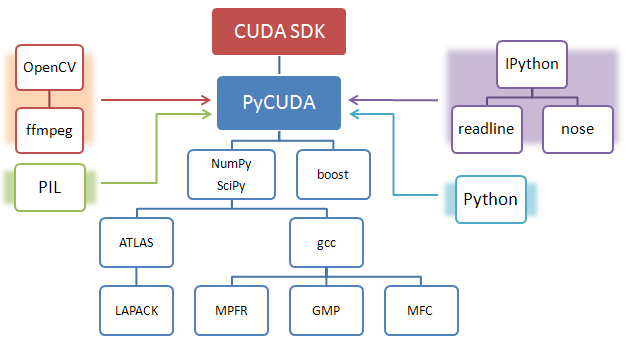
\includegraphics[width=.8\textwidth]{installedDependecies.png}
      \caption{Un posible esquema de dependencias de PyCUDA}
    \end{center}
  \end{figure}
\end{frame}

\begin{frame}[fragile]
\frametitle{Computación con Python y CUDA}

  Flujo de ejecución de PyCUDA:
  \begin{itemize}
    \item Inclusión de las librerías necesarias.
    \begin{lstlisting}
import pycuda.autoinit
import pycuda.driver as cuda
from pycuda.compiler import SourceModule
    \end{lstlisting}
   
    \item Carga de los datos en memoria.
    \begin{lstlisting}
import numpy
a = numpy.random.rand(4, 4).astype(numpy.float32)
    \end{lstlisting}

    \item Reserva de espacio en el dispositivo.
    \begin{lstlisting}
a_gpu = cuda.mem_alloc(a.nbytes)
    \end{lstlisting}

  \end{itemize}

\end{frame}

\begin{frame}[fragile]
\frametitle{Computación con Python y CUDA}
  \begin{itemize}
    \item Transferencia de datos al dispositivo.
    \begin{lstlisting}
cuda.memcpy_htod(a_gpu, a)
    \end{lstlisting}
   
    \item Ejecución del \emph{kernel}.
    \begin{lstlisting}
func = mod.get_function("kernel_name")
func(a_gpu, block=(4, 4, 1))
    \end{lstlisting}

    \item Transferencia al \emph{host}.
    \begin{lstlisting}
a_doubled = numpy.empty_like(a)
cuda.memcoy_dtoh(a_doubled, a_gpu)
    \end{lstlisting}

  \end{itemize}
\end{frame}

\begin{frame}{Computación con Python y CUDA}
  \begin{itemize}
    \item Alto nivel de abstracción.
    \item Hasta ahora, la mayoría de los dispositivos solo soportaban precisión simple.
    \item Python (lenguaje interpretado) + PyCUDA (\emph{wrapper}) inducen un cierto \emph{overhead} respecto a la ejecución \\* nativa en C.
  \end{itemize}
\end{frame}


\begin{frame}{Computación con Python y CUDA}
  \begin{figure}
    \begin{center}
      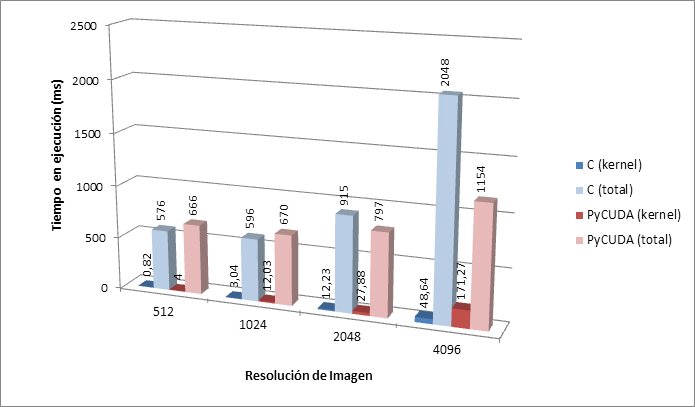
\includegraphics[width=.8\textwidth]{overhead-convolucion.png}
      \caption{Comparativa entre C y Python sobre un filtro de convolución}
    \end{center}
  \end{figure}
\end{frame}


\subsection{PyCUBLAS}

\begin{frame}{Computación con Python y CUDA}
  \begin{itemize}
    \item BLAS (Basic Linear Algebra Subprograms) es una interfaz estándar publicada en 1979.
    \item Numerosos fabricantes de hardware han creado versiones altamente optimizadas.
    \item CUBLAS es la implementación incluida por NVIDIA en el SDK de CUDA.
    \item PyCUBLAS es un \emph{wrapper} de Python para CUBLAS desarrollado por Derek Anderson.
  \end{itemize}
\end{frame}

\begin{frame}[fragile]
\frametitle{Computación con Python y CUDA}
  Ejemplo de multiplicación de matrices con PyCUBLAS:    
  \begin{lstlisting}
import numpy as np
from pycublas import CUBLASMatrix

a = np.random.randn(width,length).astype(np.float32)
b = np.random.randn(width,length).astype(np.float32)

a = CUBLASMatrix(np.mat(a))
b = CUBLASMatrix(np.mat(b))

c = a * b
  \end{lstlisting}
\end{frame}

\begin{frame}{Computación con Python y CUDA}
  \begin{figure}
    \begin{center}
      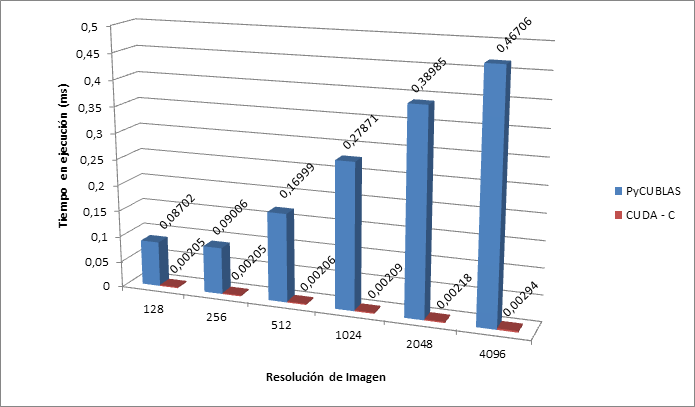
\includegraphics[width=.8\textwidth]{pycublas.png}
      \caption{Comparativa entre CUDA C y PyCUBLAS sobre la multiplicación de matrices cuadradas}
    \end{center}
  \end{figure}
\end{frame}

\section{Caso práctico: Detección de movimiento}

\subsection{Algoritmo}

\begin{frame}{Caso práctico: Detección de movimiento}
\begin{enumerate}
   \item Conversión a escala de grises de las 2 imágenes.
   \item Aplicación del filtro de diferencia a las 2 imágenes.
   \item Aplicación del filtro Threshold.
   \item Aplicación del filtro de Erosión.
   \item Mezcla en el canal R de la imagen original con la imagen resultado de los filtros.
\end{enumerate}
\end{frame}

\begin{frame}{Caso práctico: Detección de movimiento}
  \begin{figure}
    \begin{center}
      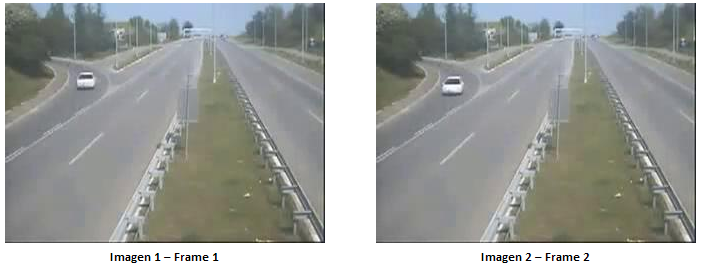
\includegraphics[width=.8\textwidth]{frames.png}
      \caption{Extracto de dos frames consecutivos del vídeo de trabajo}
    \end{center}
  \end{figure}
\end{frame}

\begin{frame}{Caso práctico: Detección de movimiento}
  \begin{figure}
    \begin{center}
      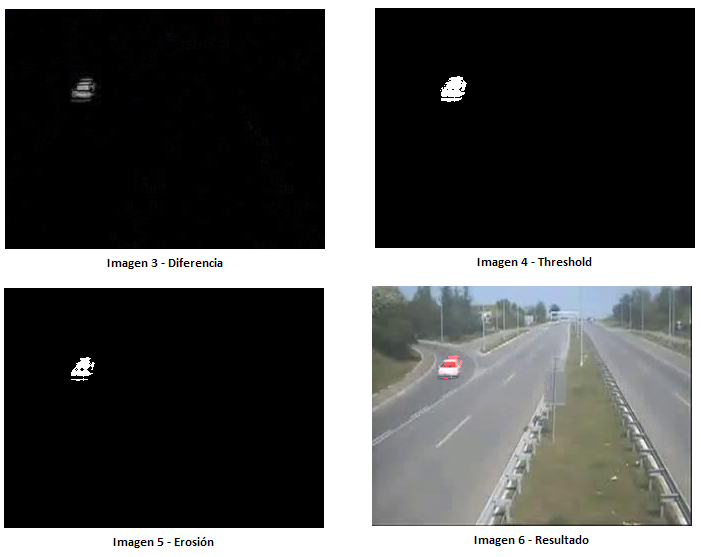
\includegraphics[width=.6\textwidth]{filters_step_by_step.png}
      \caption{Aplicación del algoritmo paso a paso}
    \end{center}
  \end{figure}
\end{frame}

\subsection{Implementación}

\begin{frame}{Caso práctico: Detección de movimiento}
  \begin{figure}
    \begin{center}
      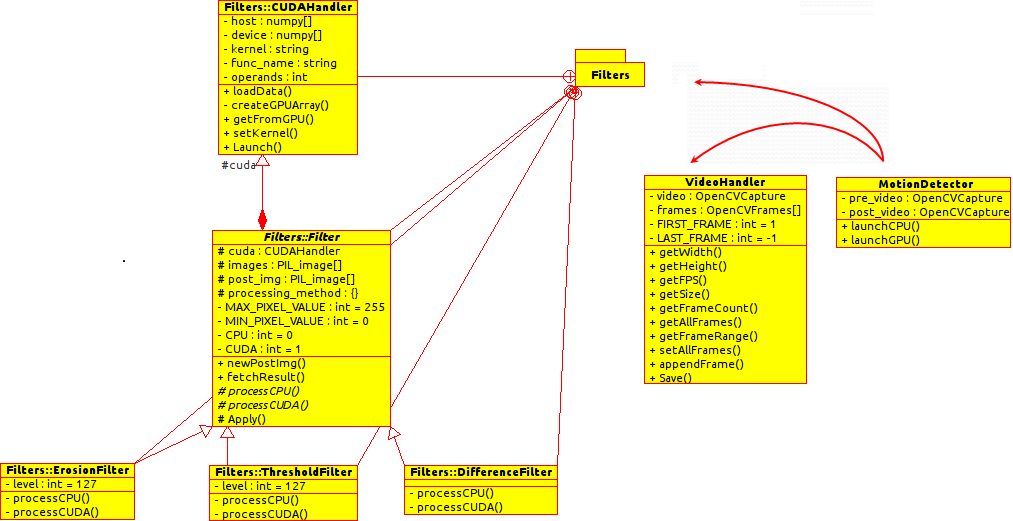
\includegraphics[width=.8\textwidth]{UML.png}
      \caption{Jerarquía de clases del detector de movimiento}
    \end{center}
  \end{figure}
\end{frame}

\begin{frame}[fragile]
\frametitle{Caso práctico: Detección de movimiento}
  \begin{mydescription}{MotionDetector}
    \item[CUDAHandler] Abstracción de la comunicación con la GPU.
    \item[VideoHandler] Abstracción de la manipulación de vídeo.
    \item[Filter] Interfaz común de la que heredan los filtros.
    \item[MotionDetector] Dirección del proceso de detección.
  \end{mydescription}

\vspace{5mm}

Ejemplo: Aplicación del filtro de diferencia
  \begin{lstlisting}
cuda.loadData(input=self.images, output=self.post_img)
from Kernels.difference_kernel import diffkernel
cuda.setKernel(diffkernel)
cuda.Launch((32, 32, 1))
  \end{lstlisting}
\end{frame}

\section{Conclusiones}

\begin{frame}{Conclusiones}
  \begin{itemize}
    \item Implementación sencilla para problemas complejos.
    \item Menor curva de aprendizaje.
    \item El \emph{overhead} inherente al uso de \emph{wrappers} y lenguajes interpretados disminuye conforme aumenta el tamaño del problema.
    \item Ideal para investigadores con necesidad de cálculo masivo paralelo.
  \end{itemize}
\end{frame}

% All of the following is optional and typically not needed. 
\appendix
% \section<presentation>*{\appendixname}
\section<presentation>*{Bibliografía destacada}

\begin{frame}[allowframebreaks]
  %\frametitle<presentation>{Bibliografía destacada}
  \frametitle{Bibliografía destacada}
    
  \begin{thebibliography}{3}
    
  \beamertemplatearticlebibitems
  % Followed by interesting articles. Keep the list short. 

   
  \bibitem{Klockner2009}
    Andreas Kl{\"o}ckner \emph{et ál.}
    \newblock PyCUDA: GPU run-time code generation for high-performance computing
    \newblock arXiv:0911.3456v2

  \bibitem{Anderson2009}
    Derek Anderson
    \newblock PyCUBLAS - Easy Python/NumPy/CUDA/CUBLAS integration
    \newblock http://kered.org

  \bibitem{Zhiyi2008}
    Zhiyi Yang, Yating Zhu, Yong Pu
    \newblock Parallel image processing based on CUDA
    \newblock CSSE (3). 2008 pp. 198-201, IEEE Computer Society
  \end{thebibliography}
\end{frame}


\section*{Preguntas}

\begin{frame}{Preguntas}
  \begin{figure}
    \begin{center}
      
\includegraphics[width=.5\textwidth]{question.jpg}
    \end{center}
  \end{figure}
\end{frame}

\section*{Agradecimientos}

\begin{frame}
  \begin{center}
    {\Huge Gracias por su atención}
  \end{center}
\end{frame}

\end{document}
